% Author: K. Potamianos <karolos.potamianos@cern.ch>
% Date: 2015-III-10

\documentclass{standalone}
\usepackage{tikz} 
\usetikzlibrary{shapes,arrows,positioning,calc,arrows.meta}

\usepackage{fontspec}
\setmainfont{Calibri}

\makeatletter
\newcommand{\gettikzxy}[3]{%
  \tikz@scan@one@point\pgfutil@firstofone#1\relax
  \edef#2{\the\pgf@x}%
  \edef#3{\the\pgf@y}%
}
\makeatother

\begin{document}

\tikzstyle{block} = [box, fill=blue!20, minimum height=3em, minimum width=6em] 
\tikzstyle{arrow} = [single arrow, draw, thick]

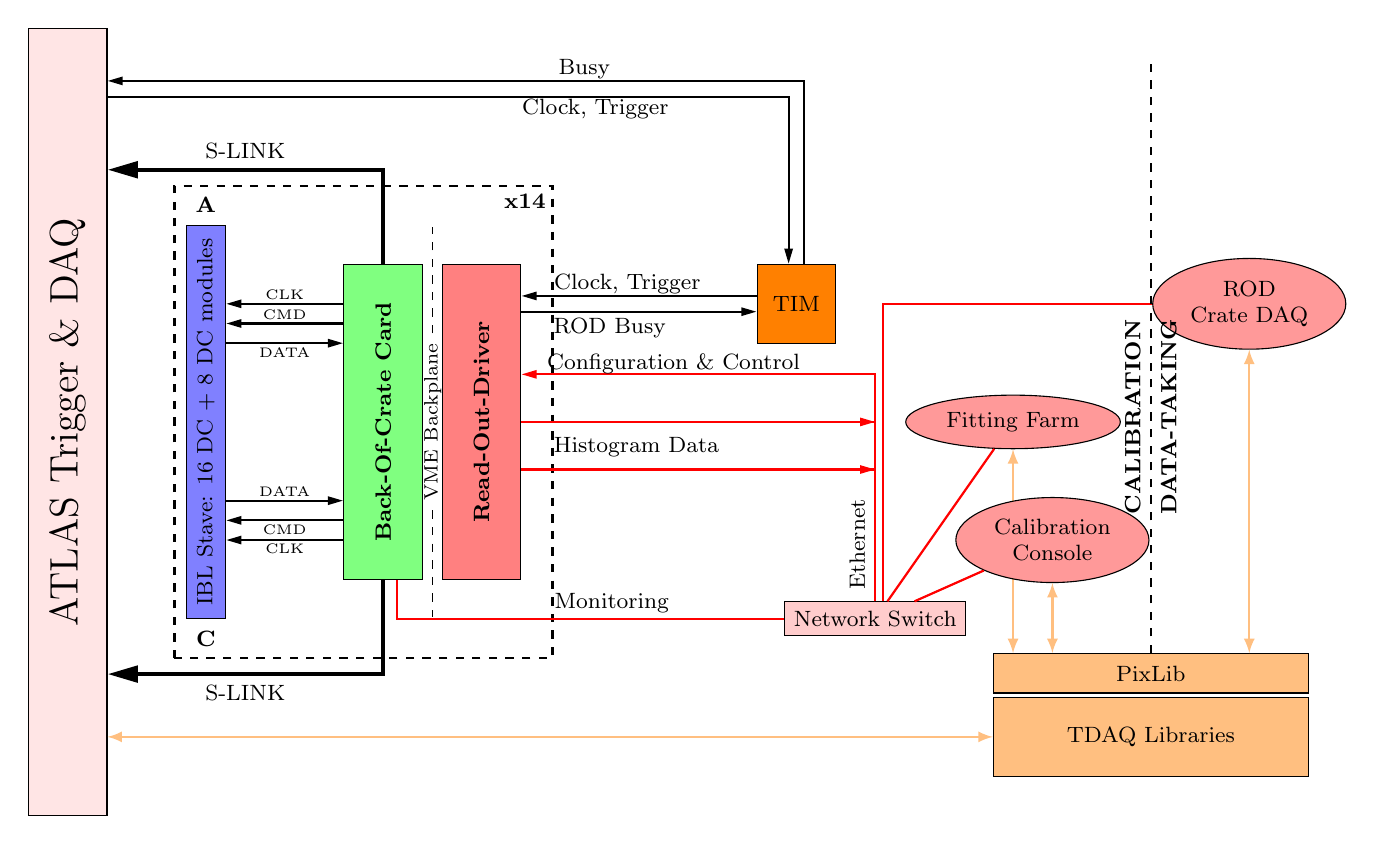
\begin{tikzpicture}[auto, node distance=0.5cm and 0.5cm, 
	arr/.style={-{Triangle[angle=30:0.2cm]},thick},
	slink/.style={ultra thick,-{Triangle[angle=30:0.4cm]}},
	line/.style= {thick},
	ttc/.style= {{Triangle[angle=30:0.2cm]}-{Triangle[angle=30:0.2cm]}},
	eth/.style={thick,red},
	box/.style={rectangle,draw=black},
	font=\footnotesize]

    \fill[transparent] (0cm,0cm) rectangle (15cm, 8cm);
%    \draw[dashed, thick] (1.9cm,1cm) rectangle (4.9cm, 7cm);
    \draw[dashed, thick] (0.1cm,1cm) rectangle (4.9cm, 7cm);
    \node at (4.55cm,6.8cm) {\bf x14};

    \node (IBL) at (.5cm,4cm) [box,fill=blue!50,minimum width=5cm, minimum height=0.5cm,rotate=90]{IBL Stave: 16 DC + 8 DC modules};
%    \node at ($(IBL.east)+(0,0.3cm)$) {\bf x14};
     \node at ($(IBL.east)+(0,0.25cm)$) {\bf A};
     \node at ($(IBL.west)-(0,0.25cm)$) {\bf C};
    
    \node (ROD) at (4cm,4cm) [box,fill=red!50,minimum width=4cm, minimum height=1cm,rotate=90]{\bf Read-Out-Driver};
    \node (BOC) at (2.75cm,4cm) [box,fill=green!50,minimum width=4cm, minimum height=1cm,rotate=90]{\bf Back-Of-Crate Card};
    \node (VME) at (3.38cm,4cm) [rotate=90] {\scriptsize VME Backplane};
    \draw [dashed] (VME.west) -- ($(VME.west) - (0,1.35cm)$);
    \draw [dashed] (VME.east) -- ($(VME.east) + (0,1.355cm)$);
    
    \draw [arr] ($(BOC.north)+(0,1.50cm)$) -- node [above,yshift=-.075cm] {\tiny CLK} ($(IBL.south)+(0,1.50cm)$);
    \draw [arr] ($(BOC.north)+(0,1.25cm)$) -- node [above,yshift=-.075cm] {\tiny CMD} ($(IBL.south)+(0,1.25cm)$);
    \draw [arr] ($(IBL.south)+(0,1.00cm)$) -- node [below,yshift=.075cm] {\tiny DATA} ($(BOC.north)+(0,1.00cm)$);

    \draw [arr] ($(BOC.north)-(0,1.50cm)$) -- node [below,yshift=.075cm] {\tiny CLK} ($(IBL.south)-(0,1.50cm)$);
    \draw [arr] ($(BOC.north)-(0,1.25cm)$) -- node [below,yshift=.075cm] {\tiny CMD} ($(IBL.south)-(0,1.25cm)$);
    \draw [arr] ($(IBL.south)-(0,1.00cm)$) -- node [above,yshift=-.075cm] {\tiny DATA} ($(BOC.north)-(0,1.00cm)$);
    
    \node (ATLAS_TDAQ) at ($(IBL.north) - (1.5cm,0cm)$) [box, fill=red!10,rotate=90,minimum width=10cm, minimum height=1cm] {\Large ATLAS Trigger \& DAQ};
    \draw [slink] (BOC.east) |- node [pos=.75,above] {S-LINK} (ATLAS_TDAQ.351);
    \draw [slink] (BOC.west) |- node [pos=.75,below] {S-LINK} (ATLAS_TDAQ.189);
    
    \node (TIM) at (8cm,5.5cm) [box, fill=orange, minimum height=1cm, minimum width=1cm] {TIM};
    \coordinate (TIM1) at ($(TIM.west) + (0,0.1cm)$);
    \coordinate (TIM2) at ($(TIM.west) - (0,0.1cm)$);
    \draw [arr] (TIM1) -- node [above,pos=.55,yshift=-0.1cm] {Clock, Trigger} (ROD.south |- TIM1);
    \draw [arr] (ROD.south |- TIM2) -- node [below,pos=0.375,yshift=0.05cm] {ROD Busy} (TIM2);
    
    \draw [arr] (ATLAS_TDAQ.353) -| node [pos=.35,above,yshift=0.1cm] {Busy} ($(TIM.north) - (0.1cm,0)$);
    \draw [arr] ($(TIM.north) + (0.1cm,0)$) |- node [pos=.65,below,yshift=-0.1cm] {Clock, Trigger} ($(ATLAS_TDAQ.353) + (0,0.2cm)$);

    \node (NET) at (9cm,1.5cm) [box, fill=red!20] {Network Switch};
    \draw [eth,arr] (NET.north) |- node [pos=.125,above,rotate=90] {\color{black} Ethernet} 
    	node [pos=.785,above,yshift=-0.125cm] {\color{black} Configuration \& Control } (ROD.320);
    \draw [eth] (NET.north) |- (ROD.south);
    \draw [eth] (NET.north) |- (ROD.220);
    \draw [eth] (BOC.185) |- node [above, pos=0.7775, above,yshift=-0.05cm] {\color{black} Monitoring} (NET.west);
    \draw [eth,arr] (ROD.220) |- node [above, pos=0.6625, yshift=0.025cm]{\color{black} Histogram Data} (ROD.220 -| NET.north);
    \draw [eth,arr] (ROD.south) |- (ROD.south -| NET.north);
    \draw [eth,] (NET.north) -- (ROD.320 -| NET.north);
       
    \node (TDAQ_LIB) at (12.5cm,0cm) [box, fill=orange!50, minimum height=1cm, minimum width=4cm] {TDAQ Libraries};
    \node (PIX_LIB) at ($(TDAQ_LIB.north) + (0,.3cm)$) [box, fill=orange!50, minimum height=0.5cm, minimum width=4cm] {PixLib};
    \draw [{latex}-{latex},orange!50,thick] (TDAQ_LIB.west) -- (ATLAS_TDAQ.south |- TDAQ_LIB.west);

    \node (FitFarm) at (10.75cm,4cm) [ellipse, draw, fill=red!40] {Fitting Farm};
    \draw [eth] (NET) -- (FitFarm);
    \draw [{latex}-{latex},orange!50,thick] (FitFarm.south) -- (FitFarm.south |- PIX_LIB.north);
    
    \node (Console) at (11.25cm,2.5cm) [ellipse, draw, fill=red!40, text width=1.5cm, text centered] {Calibration \\ Console};
    \draw [eth] (NET) -- (Console);
    \draw [{latex}-{latex},orange!50,thick] (Console.south) -- (Console.south |- PIX_LIB.north);

    \node (RCD) at (13.75cm,5.5cm) [box, ellipse, draw, fill=red!40,text width=1.5cm, text centered] {ROD Crate DAQ};
    \draw [{latex}-{latex},orange!50,thick] (RCD.south) -- (RCD.south |- PIX_LIB.north);
    \draw [eth] ($(NET.north) + (0.1cm,0)$) |- (RCD);
    
    \draw [dashed, thick] (PIX_LIB.north) -- node [above,rotate=90,pos=.4] {\bf CALIBRATION}  node [below,rotate=90, pos=.4] {\bf DATA-TAKING} ($(PIX_LIB.north) + (0,7.5cm)$);

\end{tikzpicture}

\end{document}
